%
% fig/pdn-quadrat.tex -- Petr-Douglas-Neumann fuer ein Viereck:
% Aus einem beliebigen Viereck A0=ABCD entsteht in zwei Stufen ein Quadrat.
% Stufe 1: Auf jeder Seite gleichschenklig-rechtwinklige Dreiecke nach aussen
% errichten, Spitzen E,F,G,H bilden A1.
% Stufe 2: Die Mittelpunkte der Seiten von A1 bilden das Quadrat A2.
%
% Beispiel:
%   A=(0,0), B=(6,1), C=(7,5), D=(1,6)
%   E=(3.5,-2.5), F=(8.5,2.5), G=(4.5,8.5), H=(-2.5,3.5)
%   M1=(6,0), M2=(6.5,5.5), M3=(1,6), M4=(0.5,0.5)
%
\begin{figure}
\centering
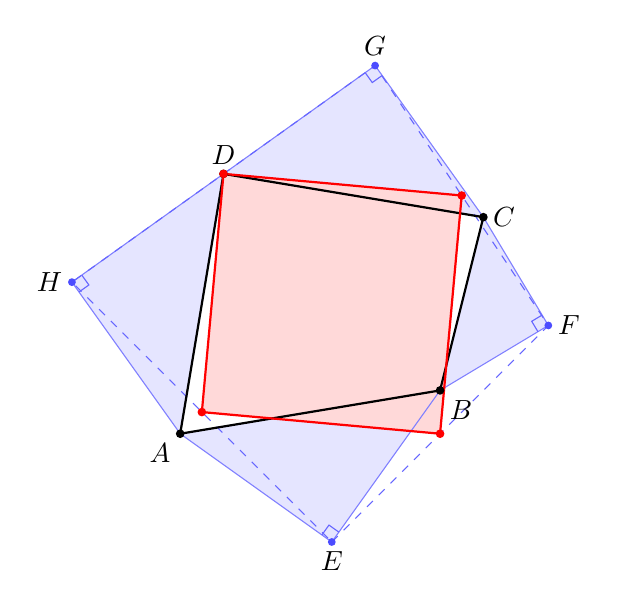
\begin{tikzpicture}[>=latex,scale=0.55]
% Ausgangsviereck A0 = ABCD (gegen den Uhrzeigersinn nummeriert)
\coordinate (A) at (0, 0);
\coordinate (B) at (6, 1);
\coordinate (C) at (7, 5);
\coordinate (D) at (1, 6);
% Spitzen der gleichschenklig-rechtwinkligen Dreiecke (Stufe 1)
\coordinate (E) at (3.5, -2.5);  % ueber AB, Spitze nach aussen
\coordinate (F) at (8.5,  2.5);  % ueber BC
\coordinate (G) at (4.5,  8.5);  % ueber CD
\coordinate (H) at (-2.5, 3.5);  % ueber DA
% Mittelpunkte der Seiten von EFGH (Stufe 2): das Quadrat A2
\coordinate (M1) at (6.0, 0.0);
\coordinate (M2) at (6.5, 5.5);
\coordinate (M3) at (1.0, 6.0);
\coordinate (M4) at (0.5, 0.5);
% Aussen errichtete rechtwinklig-gleichschenklige Dreiecke (schwach blau)
\fill[blue!10] (A) -- (B) -- (E) -- cycle;
\fill[blue!10] (B) -- (C) -- (F) -- cycle;
\fill[blue!10] (C) -- (D) -- (G) -- cycle;
\fill[blue!10] (D) -- (A) -- (H) -- cycle;
% Quadrat A2 (rot ausgefuellt)
\fill[red!15] (M1) -- (M2) -- (M3) -- (M4) -- cycle;
% Konturen der aussen errichteten Dreiecke
\draw[blue!50,thin] (A) -- (E) -- (B);
\draw[blue!50,thin] (B) -- (F) -- (C);
\draw[blue!50,thin] (C) -- (G) -- (D);
\draw[blue!50,thin] (D) -- (H) -- (A);
% Viereck EFGH = A1 (gestrichelt, dezent)
\draw[blue!60,thin,dashed] (E) -- (F) -- (G) -- (H) -- cycle;
% Ausgangsviereck A0 = ABCD (kraeftig schwarz)
\draw[thick] (A) -- (B) -- (C) -- (D) -- cycle;
% Quadrat A2 (kraeftig rot)
\draw[red,thick] (M1) -- (M2) -- (M3) -- (M4) -- cycle;
% Rechte-Winkel-Markierungen an E, F, G, H (kleine Quadrate)
\draw[blue!60,thin]
  (3.272,-2.337) -- (3.435,-2.109) -- (3.663,-2.272);
\draw[blue!60,thin]
  (8.260, 2.356) -- (8.116, 2.596) -- (8.356, 2.740);
\draw[blue!60,thin]
  (4.663, 8.272) -- (4.435, 8.109) -- (4.272, 8.337);
\draw[blue!60,thin]
  (-2.272,3.663) -- (-2.109,3.435) -- (-2.337,3.272);
% Punkte
\foreach \p in {A,B,C,D} \fill (\p) circle (0.10);
\foreach \p in {E,F,G,H} \fill[blue!70] (\p) circle (0.09);
\foreach \p in {M1,M2,M3,M4} \fill[red] (\p) circle (0.10);
% Beschriftungen
\node at (A)  [below left]  {$A$};
\node at (B)  [below right] {$B$};
\node at (C)  [right]       {$C$};
\node at (D)  [above]       {$D$};
\node at (E)  [below]       {$E$};
\node at (F)  [right]       {$F$};
\node at (G)  [above]       {$G$};
\node at (H)  [left]        {$H$};
\end{tikzpicture}
\caption{Petr-Douglas-Neumann-Theorem für ein Viereck am Beispiel
$A = 0$, $B = 6 + i$, $C = 7 + 5i$, $D = 1 + 6i$.
Über jeder Seite des Vierecks $ABCD$ (schwarz) wird ein
gleichschenklig-rechtwinkliges Dreieck (rechter Winkel an der Spitze,
markiert) nach aussen errichtet (blau);
die Spitzen $E$, $F$, $G$, $H$ bilden das Viereck $A_1$ (gestrichelt).
Die Mittelpunkte der Seiten von $A_1$ bilden das Quadrat $A_2$ (rot) ---
das Resultat des Verfahrens für $n = 4$.
\label{komplex:figure:pdn-quadrat}}
\end{figure}
